\documentclass{article}
\usepackage{utils}

\usepackage{physics}
\usepackage{amsthm,amsfonts,amsmath}

\theoremstyle{definition}
\newtheorem{example}{Пример}


\title{Quantum Machine Learning}
\date{}

\begin{document}

\maketitle

\section{Введение}
В данном документе содержит введение в квантовые вычисления, основные алгоритмы и их применение в машинном обучении.


\subsection{Квантовый компьютер}

Квантовый компьютер --- это вычислительное устройство, которое использует некоторые явления квантовой механики
(суперпозиция состояний (superposition), квантовая запутанность (entanglement)).
Квантовые компьютеры могут решать некоторые задачи значительно быстрее классических архитектур за счет того,
что все операции выполняются сразу над всеми возможными состояниями системы.

\subsection{Кубиты}
В классической архитектуре информация представляется битами, которые могут принимать только одно из двух значений:
$0$ или $1$.
В системе из $L$ битов, соответсвенно, может быть $2^L$ различных состояний.
Как правило, при выполнении операций с системой мы производим операции с одним (может быть несколькими) состоянием системы.

В квантовом же компьютере аналогом бита является квантовый бит --- кубит.
Это некоторая квантовая система, обладающая двумя базисными состояниями ($\ket{0}$ и $\ket{1}$).
Система из $L$ кубитов обладает $2^L$ базисными состояниями.

\begin{example}
При $L = 3$ получаем следующие состояния:
$\ket{000}$, $\ket{001}$, $\ket{010}$, $\ket{011}$, $\ket{100}$, $\ket{101}$, $\ket{110}$, $\ket{111}$.
\end{example}

Для удобства в дальнейшем состояния системы будем обозначать $\ket{j}, j=\overline{1, N}, N = 2^L$.
Общее состояние системы описывается {\em суперпозицией} ее базисных состояний
\[
    \ket{\psi} = \sum_{j=1}^{N} \lambda_j \ket{j}, \quad \sum_{j=1}^N |\lambda_j|^2 = 1,
\]
где $\lambda_j \in \mathbb{C}$ --- это комплексные амплитуды.

\subsection{Базовые операции}

Пространством состояний квантовой системы является $2^L$-мерное гильбертово пространство
(или $N$-мерное в наших обозначениях).
Базовые состояния $\{\ket{j}\}_{j=1}^N$ образуют ортонормироанный базис.
Обозначение $\ket{v}$ соответствует вектор-столбцу $v$, а $\bra{v}$ --- его эрмитово сопряжению $v^\dag$
\[
    v = \begin{pmatrix}
    a_1 \\
    \cdots \\
    a_N 
    \end{pmatrix},
    \quad
    v^\dag = \begin{pmatrix} \overline{a_1} & \cdots & \overline{a_N} \end{pmatrix}.
\]
Тогда скалярное произведение векторов $v, u$ может быть записано как $\bra{v}\ket{u}$.

Над системой можно проводить два типа операций:
\begin{enumerate}
    \item Измерение.
    \item Унитарное преобразование.
\end{enumerate}

\paragraph*{Измерение.}
Едиснтвенный способ получить информацию о состоянии системы это провести операцию {\em измерение}.
Измерение возвращает случайную величину, которая принимает одно из значений $\ket{j}, j=\overline{1, N}$
с вероятностью $|\lambda_j|^2$.
Эта операция необратима, то есть повторное измерение вернет то же самое состояние системы.
Поэтому в квантовых системах нет условных операций \texttt{if ... else ...} (хотя есть некоторые условные операции, например, вентилем controlled-NOT или CNOT, подробнее смотри в следующих разделах).
Спонтанные измерения системы вносят неустойчивость и создают трудности в создании систем с большим количеством кубитов.

Математическим языком измерения описываются следующим образом.
Пусть $P_S \colon V \rightarrow S$ проектор из множества всех возможных состояний системы $V$
на некоторое его подмножество $S$.
Запишем $\ket{v} = s_1 + s_2$, где $s_a \in S, s_2 \in S^\bot$.
Тогда $P_S\ket{v}$ вернет состояние $\ket{v}$ с вероятностью $|P_S\ket{v}|^2$.
Заметим, что $\ket{v}$ не обязательно базисный вектор $\ket{j}$, а некоторая суперпозиция базисных векторов.
Этим можно пользоваться для проведения менее тривиальных измерений.

\begin{example}[Проверка на совпадение битов]
    Рассмотрим систему из двух кубитов.
    В этой системе $\ket{v} = a_{00}\ket{00} + a_{01}\ket{01} + a_{10}\ket{10} + a_{11}\ket{11}$
    Пусть $S_1 = span(\ket{00}, \ket{11})$.
    Тогда проектор $P_{S_1}$ с вероятностью $a_{00}^2 + a_{11}^2$ вернет вектор из $S_1$,
    в котором оба биты одинаковые.
    При этом мы не будем знать точные значения битов, а только то, что они совпадают.
\end{example}

Для дальнейшего удобства обычно используют самосопряженные операторы для обозначения измерений
(Это можно делать, так как для любого разложения пространства $V$ в прямую сумму подпространств существует
самосопряженный оператор, $\sum_{j=1}^k \lambda_j P_j$ --- самоспряженный оператор).
Заметим, что не все самосопряженные операции одинаково легко реализуемы на практике с точки зрения физической реализации.


\paragraph*{Унитарные преобразования.}
Так как квадрат модуля комплексной амплитуды показывает вероятность оказаться в соответствующем состоянии,
а вероятности должны суммироваться в $1$,
то с системой можно производить только унитарные преобразования
(неунитарные преобразования запрещены).
Кроме того, унитарные преобразования гарантируют обратимость каждого шага алгоритма.

Из унитарности преобразований вытекает правило (no-cloning): нельзя копировать состояния подсистемы,
то есть не существует такого оператора $U$, что для любого $\ket{a}$ выполнялось бы $U\ket{a}{0} = \ket{a}\ket{a}$.
Хотя отдельные операции копирования все же существуют
(например, $a\ket{0} + b|\ket{1} \rightarrow a\ket{0\ldots0} + b\ket{1\ldots1}$).

Любые преоразования $n$-кубитной системы могут представлены в виде композиции 
$1$- и $2$-кубитных преобразований.
Такие преобразования называются {\em квантовыми вентилями} (quantum gates),
а композиции этих преобразований --- {\em квантовыми цепями} (quantum gate arrays или quantum circuits).
%
\textbf{Преобразования Паули}:
\begin{enumerate}
    \item $I = \ket{0}\bra{0} + \ket{1}\bra{1} = \begin{pmatrix}
        1 & 0 \\
        0 & 1\\
    \end{pmatrix}$.
    \item $X = \ket{0}\bra{1} + \ket{1}\bra{0} = \begin{pmatrix}
        0 & 1 \\
        1 & 0 \\
    \end{pmatrix}$ --- замена $\ket{0}$ на $\ket{1}$ и наоборот (аналог операции \texttt{NOT}).
    \item $Y = XZ = \ket{0}\ket{1} - \ket{1}\ket{0} = \begin{pmatrix}
    0 & 1 \\
    -1 & 0 \\
    \end{pmatrix}$.
    \item $Z = \ket{0}\bra{0} - \ket{1}\bra{1} = \begin{pmatrix}
    1 & 0 \\
    0 & -1 \\
    \end{pmatrix}$ --- сдвиг фазы.
\end{enumerate}
%
\textbf{Преобразование Адамара}
\begin{enumerate}
    \item[5] $H = \frac{1}{\sqrt{2}}\left (
    \ket{0}\bra{0} + \ket{0}\bra{1} + \ket{1}\bra{0} - \ket{1}\bra{1}
    \right ) = \frac{1}{\sqrt{2}}\begin{pmatrix}
        1 & 1 \\
        1 & -1 \\
    \end{pmatrix}$ или \\
    $H \colon \begin{cases}
    \ket{0} \rightarrow \frac{1}{\sqrt{2}} \left (
        \ket{0} + \ket{1}
    \right ) = \ket{+}, \\
    \ket{1} \rightarrow \frac{1}{\sqrt{2}} \left (
        \ket{0} - \ket{1}
    \right ) = \ket{-}.
    \end{cases}$
\end{enumerate}
%
\textbf{Controlled NOT}
\begin{enumerate}
    \item[6] $C_{not} = \ket{00}\bra{00} + \ket{01}\bra{01} + \ket{10}\bra{11} + \ket{11}\bra{10} = 
    \begin{pmatrix}
    1 & 0 & 0 & 0 \\
    0 & 1 & 0 & 0 \\
    0 & 0 & 0 & 1 \\
    0 & 0 & 1 & 0 \\
    \end{pmatrix}$.\\
    Оператор изменяет второй бит, если первый бит равен $1$.
    $C_{not}$ является обратным самому себе.
    Эта операция делает 2 независимых кубита запутанными и наоборот, так как обратна сама себе.\\
    \textbf{Замечание:} при применении к запутанным состояниям контроль может изменяться.
    Кроме того, вместо операции NOT можно выполнять произвольное унитароное преобразование $U$
    (тогда вентиль называется controlled-$U$).
\end{enumerate}

Данные операции используются для построения обратимых квантовых версий классических логических операций
(подробнее можно посмотреть в
\href{http://csis.pace.edu/ctappert/cs837-19spring/Rieffel-Quantum%20Computing.pdf}{Quantum computing. A gentle introduction.}).



\begin{example}[Алгоритм Дойча]
Для функции $f \colon \{0, 1\} \rightarrow \{0, 1\}$ определить, является ли она константной.
Любой классический алгоритм решает эту задачу за 2 вызова функции.
Квантовый алгоритм делает это за один вызов функции.

Пусть $U_f$ --- это унитарное преобразование над двух-кубитной системой,
$U_f \colon \ket{x}\ket{y} \rightarrow \ket{x}\ket{y \oplus f(x)}$.
Тогда 
\begin{align*}
U_f(\ket{+}\ket{-})
&=
\frac12\sum_{x=0}^1 \ket{x}(\ket{0 \oplus f(x)} - \ket{1 \oplus f(x)}) 
= \left |
\frac{1}{\sqrt{2}}(\ket{0 \oplus f(x)} - \ket{1 \oplus f(x)}) = (-1)^{f(x)}\ket{-}
\right | \\
&= \sum_{x=0}^1 (-1)^{f(x)} \ket{x} \ket{-}.
\end{align*}
При $f(x) = const$ получаем $\pm \ket{+}\ket{-}$, в противном случае --- $\pm \ket{-}\ket{-}$.
Применяя преобразование Адамара к первому кубиту, а затем измеряя его, мы гарантированно получим
$1$ в случае постоянной функции, и $0$ в противном случае.

Обобщение на случай, когда на вход подается $n$ бит, а на выходе один бит, тоже решается за один вызов $U_f$.
\end{example}

\subsection{Квантовое преобразование Фурье и оценка фазы}
Квантовое преобразование Фурье следующим образом преобразует базовые состояния
\[
\ket{j} \rightarrow \frac{1}{\sqrt{N}} \sum_{k=0}^{N-1} e^{2\pi ijk / N} \ket{k}.
\]
Пусть $j = j_1 j_2 \ldots j_n$ --- битовое представление числа $j$.
Введем также обозначение $0.j_1 j_2 \ldots j_n = j_1 / 2 + j_2 / 4 + \cdots + j_n / 2^n$.
Тогда преобразование Фурье можно представить в виде
\[
\ket{j} \rightarrow \frac{(\ket{0} + e^{2\pi i 0.j_n}\ket{1}) \cdots
                          (\ket{0} + e^{2\pi i 0.j_1 \ldots j_n} \ket{1})}{2^n}.
\]
Из выражения становится понятно, какие вентили надо использовать для построения цепи
(см. Рис.\ref{fig:fourier_transform}):
сначала вентиль $H$ (преобразование Адамара для перехода к $\ket{0} \pm \ket{1}$),
а затем controlled-$R_k$ вентиль, где $R_k$ делает сдвиг фазы во втором кубите:
\[
R_k = \begin{pmatrix}
    1 & 0 \\
    0 & e^{2\pi i / 2^k}.
\end{pmatrix}
\]

\begin{figure}[H]
    \centering
    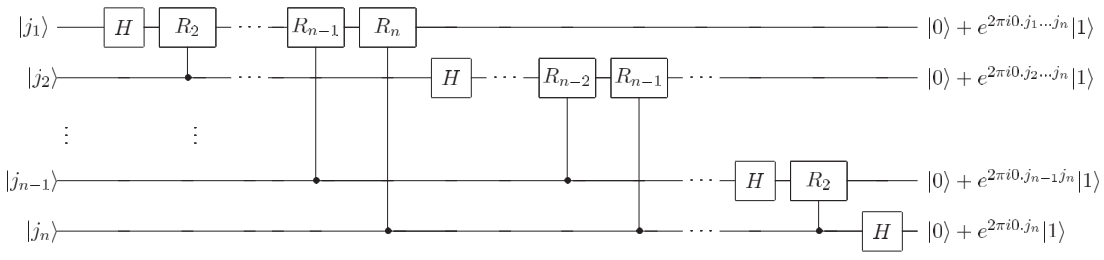
\includegraphics[width=\textwidth]{figures/fourier_transform.png}
    \caption{Схема вычисления преобразования Фурье.
    Черные точки обозначают управляющее состояние для controlled-операций}
    \label{fig:fourier_transform}
\end{figure}


% 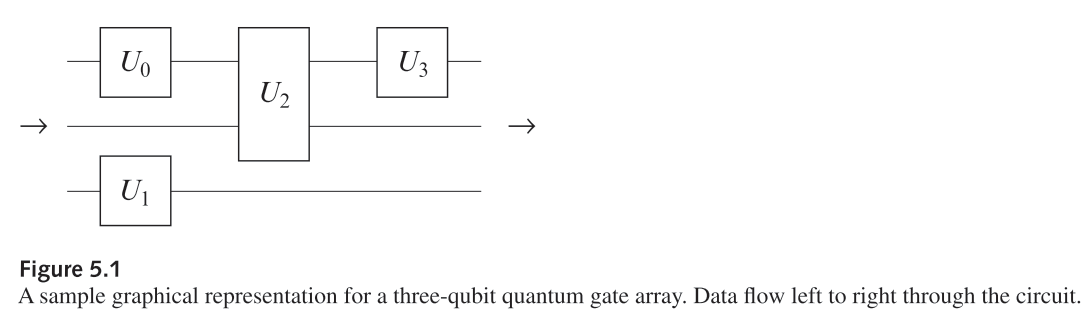
\includegraphics{figures/quantum_gate.png}

\end{document}